\usetikzlibrary{arrows.meta,shapes.multipart}

\begin{frame}{address split diagram}
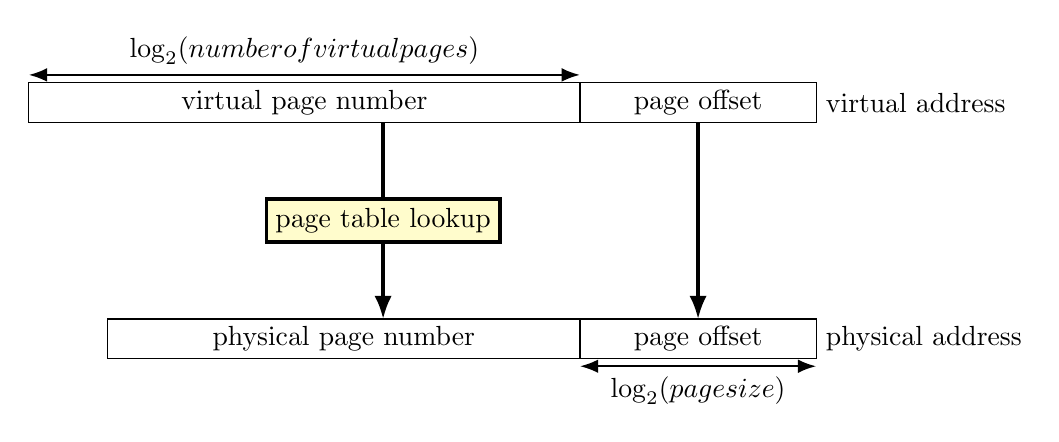
\begin{tikzpicture}
    \draw (0,0) rectangle ++(7, -.5) node[midway] {virtual page number};
    \draw (7,0) rectangle ++(3, -.5) node[midway] {page offset};
    \node[anchor=west] at (10, -.25) {virtual address};
    \draw (1,-3) rectangle ++(6, -.5) node[midway] {physical page number};
    \draw (7,-3) rectangle ++(3, -.5) node[midway] {page offset};
    \draw[very thick,-Latex] (4.5, -.5) -- (4.5, -3)
        node[midway,draw,fill=yellow!20] {page table lookup};
    \draw[very thick,-Latex] (8.5, -.5) -- (8.5, -3);
    \node[anchor=west] at (10, -3.25) {physical address};
    \draw[Latex-Latex,thick] (7, -3.6) -- ++(3, 0)
        node[midway,below] {$\log_2(\text{page size})$};
    \draw[Latex-Latex,thick] (0, 0.1) -- ++(7, 0)
        node[midway,above] {$\log_2(\text{number of virtual pages})$};
\end{tikzpicture}
\end{frame}
